\documentclass[tikz,border=1.35mm]{standalone}

\definecolor{splitred}{HTML}{AF2525}

% Face-based isotropic refinement skeleton for a tetrahedral cell.
% Red nodes are edge midpoints, face centroids, and the element centroid.
\begin{document}
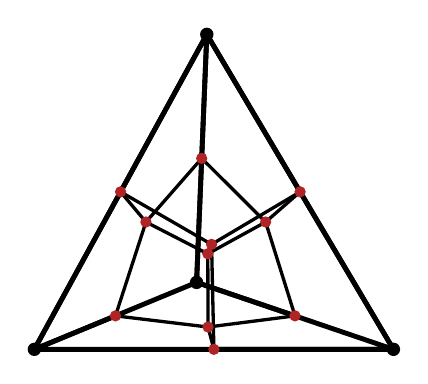
\begin{tikzpicture}[
  x={(19mm,0mm)},
  y={(7mm,4mm)},
  z={(0mm,18mm)},
  line join=round,
  line cap=round,
  edge/.style={draw=black,line width=0.62mm},
  split/.style={draw=black,line width=0.42mm}
]
  % Original vertices.
  \coordinate (v0) at (0,0,0);
  \coordinate (v1) at (2.4,0,0);
  \coordinate (v2) at (0.55,1.45,0.15);
  \coordinate (v3) at (0.95,0.55,2.1);

  % Edge midpoints.
  \coordinate (m01) at (1.2,0,0);
  \coordinate (m12) at (1.475,0.725,0.075);
  \coordinate (m20) at (0.275,0.725,0.075);
  \coordinate (m03) at (0.475,0.275,1.05);
  \coordinate (m13) at (1.675,0.275,1.05);
  \coordinate (m23) at (0.750,1.000,1.125);

  % Face centroids and element centroid.
  \coordinate (f012) at (0.983,0.483,0.050);
  \coordinate (f013) at (1.117,0.183,0.700);
  \coordinate (f123) at (1.300,0.667,0.750);
  \coordinate (f203) at (0.500,0.667,0.750);
  \coordinate (center) at (0.975,0.500,0.563);

  % Split outer faces: each face centroid connects to its edge midpoints.
  \draw[edge] (v0) -- (m01) -- (v1) -- (m12) -- (v2) -- (m20) -- cycle;
  \draw[edge] (v0) -- (m03) -- (v3) -- (m13) -- (v1) -- (m01);
  \draw[edge] (v1) -- (m13) -- (v3) -- (m23) -- (v2) -- (m12);
  \draw[edge] (v2) -- (m23) -- (v3) -- (m03) -- (v0) -- (m20);

  \draw[split] (f012) -- (m01);
  \draw[split] (f012) -- (m12);
  \draw[split] (f012) -- (m20);
  \draw[split] (center) -- (f012);

  \draw[split] (f013) -- (m01);
  \draw[split] (f013) -- (m13);
  \draw[split] (f013) -- (m03);
  \draw[split] (center) -- (f013);

  \draw[split] (f123) -- (m12);
  \draw[split] (f123) -- (m23);
  \draw[split] (f123) -- (m13);
  \draw[split] (center) -- (f123);

  \draw[split] (f203) -- (m20);
  \draw[split] (f203) -- (m03);
  \draw[split] (f203) -- (m23);
  \draw[split] (center) -- (f203);

  % Original vertices are black; refinement-created nodes are red.
  \foreach \p in {v0,v1,v2,v3} {
    \fill[black] (\p) circle[radius=0.85mm];
  }
  \foreach \p in {m01,m12,m20,m03,m13,m23,f012,f013,f123,f203,center} {
    \fill[splitred] (\p) circle[radius=0.72mm];
  }
\end{tikzpicture}
\end{document}
